\chapter{String Tension, Planck Units, and the Easy Version of Twenty-Six Dimensions}

These notes follow Leonard Susskind's fifth lecture on string theory, with visual curation by LazyingArt LLC and Video2Book. The lecture falls naturally into two acts. First he repairs an omission from the earlier meetings: we have talked about strings without really talking about units, and from that omission emerges the one physical scale in the problem, the string tension. Only after that long first act, with its talk of Planck units, direct detectability, unification, and black holes, does he reset and give the old heuristic argument for why bosonic string theory seems to want twenty-six spacetime dimensions. The point of the chapter is to let that motion remain visible on the page.

\section{From Hooke's Law to the One Scale in the Problem}

Susskind begins with a question that sounds almost embarrassingly basic: if a hadron is a string, and if we excite it by rotation or vibration, what sets the gap between the ground state and the first excited state? In this theory, he says, there is really only one parameter, so the right way to find it is to go back to the simplest picture of a stretched string.

\begin{figure}[t]
\centering

\includegraphics[width=0.72\textwidth]{lecture_05_figure_02.png}
\caption{Hooke-law potential for a stretched string. The board writes the endpoint separation as \(X\); later in the lecture the same separation is relabeled by \(\ell\).}
\end{figure}

The board first gives the familiar spring-law energy,
\begin{equation}
E=\frac{KX^{2}}{2}.
\end{equation}
That is just Hooke's law written for the distance between the endpoints. In the live lecture the factor of \(1/2\) is restored on the fly, and the symbol \(X\) later becomes \(x\) and then \(\ell\). In cleaned notation we therefore write
\begin{equation}
E=\frac{k\ell^{2}}{2}.
\end{equation}

At this stage nothing has yet become specifically string-theoretic. We simply have an ordinary nonrelativistic string, or if one prefers, an idealized rubber band, whose potential energy is quadratic in its extension. But the lecture is not really interested in this formula for its own sake. He is using it to isolate the one scale that controls the theory.

\section{Why the Relevant Scale Is Mass Squared}

The first genuine pivot comes immediately. The nonrelativistic energy in the stretched string is not being identified with the mass of the string. In the fast-moving, infinite-momentum description that has been used in earlier lectures, the internal nonrelativistic energy is identified with the square of the mass:
\begin{equation}
m^{2}\propto k\ell^{2}.
\end{equation}
That is the reason the spring-law discussion matters here. Taking the square root, and suppressing inessential factors such as \(\sqrt{2}\) just as Susskind does, we get
\begin{equation}
m\propto \sqrt{k}\,\ell.
\end{equation}

This tells us what the physically meaningful parameter is. The square root of the spring constant is the tension:
\begin{equation}
T=\sqrt{k}.
\end{equation}
Once that is said, the rest-frame interpretation is immediate:
\begin{equation}
E_{\text{rest}}\sim T\,\ell.
\end{equation}
So the mass or rest energy of a stretched string is proportional to its length, with the coefficient of proportionality equal to the tension. It is exactly like surface tension in spirit, except that now the object is one-dimensional.

The lecture then pauses to ask what units this quantity has. In units with \(c=\hbar=1\),
\begin{equation}
[E]=L^{-1},
\end{equation}
so the tension, being energy per unit length, has dimensions
\begin{equation}
[T]=L^{-2}.
\end{equation}
Equivalently, it has dimensions of energy squared. This is already the answer to the original question about excitation gaps. The natural unit in string theory is a unit of mass squared, and each time the string is excited by one oscillator quantum, it adds essentially one unit of tension to \(m^{2}\).

Susskind then reinforces the point with the ordinary harmonic oscillator. For a spring of unit mass,
\begin{equation}
\omega\sim \sqrt{\frac{k}{m}}\sim \sqrt{k},
\end{equation}
and the energy gap between successive oscillator levels is proportional to \(\omega\). So the stronger the spring, the larger the frequency; the larger the frequency, the larger the excitation gap. The string is no different in spirit. Once the tension is known, the scale of the spectrum is known.

There is also a more tangible way to say what tension means. It is energy per unit length, and energy per unit length is force. If one imagines suspending a weight from a string in a gravitational field, the tension is the weight the string can support. Since \(E_{\text{rest}}\sim T\ell\), the supportable force is independent of the length of the string. In the hadronic case the lecture puts the number at the level of a truck. Nobody, of course, has ever literally hung a truck from a meson; the point is that we infer the hadronic tension from the observed excitation energies, and from that inferred tension we can tell how strong the string would be. Fundamental strings, if they underlie gravitons and electrons, must be far stronger still.

\section{Planck Units and the Scale of Fundamental Strings}

Now the lecture widens its scope. Hadronic strings are already strong, but the strings of fundamental string theory would have vastly greater tension. They would be stiffer, harder to excite, and smaller in their ground-state fluctuations. That leads naturally to the next question: what scale should we compare them to? Susskind's answer is the Planck scale, but he does not simply quote it. He works it out.

The real issue, as he presents it, is not only numerical. Our laboratory units are biologically or historically convenient, but they are not fundamental. A meter is a useful human length, a kilogram a useful laboratory mass, a second a useful pendulum-like interval. A fundamental theory should instead use truly universal constants. The lecture therefore chooses
\begin{equation}
[c]=LT^{-1},
\qquad
[\hbar]=ML^{2}T^{-1},
\qquad
[G]=L^{3}M^{-1}T^{-2}.
\end{equation}

He deliberately starts with length squared rather than length, partly to avoid an unnecessary square root and partly because, as he briefly remarks, it may even be that area is in some sense the more primitive quantity. So we seek powers \(p,q,r\) such that
\begin{equation}
G^{p}\hbar^{q}c^{r}
\end{equation}
has dimensions of \(L^{2}\). Matching powers of \(M\), \(T\), and \(L\) gives
\begin{align}
-p+q&=0,\\
-2p-q-r&=0,\\
3p+2q+r&=2.
\end{align}
The mass equation gives \(q=p\), the time equation gives \(r=-3p\), and the length equation then yields \(2p=2\), so \(p=1\). Thus
\begin{equation}
\ell_{P}^{2}=\frac{G\hbar}{c^{3}}.
\end{equation}
That is the Planck area. From it one defines the Planck length
\begin{equation}
\ell_{P}=\sqrt{\frac{G\hbar}{c^{3}}},
\end{equation}
the Planck time by light-crossing,
\begin{equation}
t_{P}=\frac{\ell_{P}}{c},
\end{equation}
and the corresponding mass scale
\begin{equation}
m_{P}=\sqrt{\frac{\hbar c}{G}}.
\end{equation}

The lecture keeps the numbers only at order-of-magnitude precision:
\begin{equation}
\ell_{P}\sim 10^{-35}\,\mathrm{m},
\qquad
t_{P}\sim 10^{-43}\,\mathrm{s},
\qquad
m_{P}\sim 10^{-8}\,\mathrm{kg}\sim 10^{19}\,\mathrm{GeV}.
\end{equation}
The contrast is the point. The Planck length and Planck time are impossibly small, while the Planck mass is not microscopic at all in everyday units: it is closer to a tiny dust grain. That is why the Planck energy sounds enormous in particle-physics language but not in gross human bookkeeping.

This is the scale Susskind then associates, at least schematically, with fundamental strings. A very stiff string has very rapid oscillations, so it has very high excitation energies; the same stiffness also suppresses ground-state fluctuations, so the string is very small. That is why the two expectations go together:
\begin{equation}
\text{string size} \sim \ell_{P},
\qquad
\text{oscillation time} \sim t_{P},
\qquad
\text{excitation energy} \sim m_{P}.
\end{equation}

\subsection{Question \& Answer}

\paragraph{Why think the string scale is near the Planck scale, and why not much smaller?}

The lecture is careful here. This is not meant as a theorem. It is a physically motivated guess, supported by several lines of thought.

First, there is the phenomenological side. Extrapolations of the standard-model couplings suggest that ordinary quantum field theory continues to work to extremely short distances, perhaps down to scales only \(10^{2}\) or \(10^{3}\) times larger than the Planck length. That does not pin the string scale down exactly, but it tells us that stringy behavior cannot be showing up at ordinary particle-physics distances.

Second, there is the black-hole obstruction to going much below the Planck length. If we try to localize degrees of freedom to a region of size
\begin{equation}
\Delta x\sim \ell_{P},
\end{equation}
then the uncertainty principle implies
\begin{equation}
\Delta p\sim \frac{\hbar}{\ell_{P}},
\end{equation}
and therefore an energy of order
\begin{equation}
E\sim c\,\Delta p\sim m_{P}c^{2}.
\end{equation}
Trying to push to still shorter lengths pushes the energy still higher. But a very small object carrying energy above the Planck scale no longer looks naturally like a string; gravity takes over, and one is driven toward black-hole formation. This is why the lecture treats sub-Planckian string lengths as physically implausible.

One should also keep the length-energy inversion straight. A string scale somewhat below the Planck \emph{energy} corresponds to a string length somewhat above the Planck \emph{length}. That mild separation is possible. What the lecture argues against is the opposite direction, namely strings much shorter than \(\ell_{P}\).

\section{How Hard Would It Be to See Stringiness Directly?}

The lecture now turns from units to phenomenology. The style becomes estimate-driven and deliberately concrete. What does it mean, physically, to say that a fundamental particle might be a string?

The answer is that one would like to detect stringiness in exactly the way hadronic physics once detected the string-like structure of hadrons: strike the object, set it vibrating, and discover a tower of excited states. In the present discussion the natural increments are increments of mass squared, and the scale of those increments is set by the tension, hence by the Planck scale. For a particle such as an electron or a graviton, the energy required to excite the first stringy mode is expected to be enormous,
\begin{equation}
m_{P}\sim 10^{19}\,\mathrm{GeV}.
\end{equation}
That is why direct excitation looks hopeless. It is not enough to have a large amount of energy in total. One must concentrate that energy into an extraordinarily small region.

Susskind makes this scale vivid with a sequence of deliberately outrageous comparisons. A hadronic string, if hung in a laboratory fantasy, could support something on the order of a truck. A fundamental string, with its much larger tension, would in the same fantasy support something on the order of a galaxy, provided one arranged the background gravitational field so that the comparison made sense. These analogies are not decorative. They are his way of turning the abstract statement ``the tension is huge'' into something one can feel.

There is another side to the same story. The more stiffly bound the string is, the smaller it is in its ground state. So if the electron really is a string, its stringy extension is not something we can simply look at under a microscope. To see it, one has to excite it.

This connects directly with gravity. In electromagnetism the force law is schematically
\begin{equation}
F_{\mathrm{em}}\sim \frac{e^{2}}{R^{2}},
\end{equation}
whereas in gravitation it is
\begin{equation}
F_{\mathrm{grav}}\sim \frac{GM^{2}}{R^{2}}.
\end{equation}
So the quantity analogous to the electromagnetic coupling is not \(G\) by itself but rather
\begin{equation}
\alpha_{\mathrm{grav}}(M)\sim GM^{2}.
\end{equation}
At low energies this is tiny. Near the Planck scale it becomes of order one. That is the sense in which gravity ``catches up'' with the other interactions.

The lecture then discusses black holes. There are, he says, two ways to make one. One is by gravitation in the ordinary macroscopic sense: let a sufficiently heavy object collapse under its own gravitational pull. The other is by kinetic concentration: smash together enough energy in a small enough volume that gravity becomes strong and forms a black hole. The first route takes stars. The second route takes Planckian collisions.

\begin{figure}[t]
\centering

\includegraphics[width=0.62\textwidth]{lecture_05_figure_03.png}
\caption{Qualitative energy sketch for gravitational collapse. The photographed board is not legible enough to support exact formulas, but it clearly organizes several competing branches and a collapse threshold.}
\end{figure}

The red board sketch shown in the lecture belongs to this discussion. It is qualitative rather than quantitative: the point is that several contributions compete, meet near a threshold, and then a sharply rising branch appears.

\begin{figure}[t]
\centering
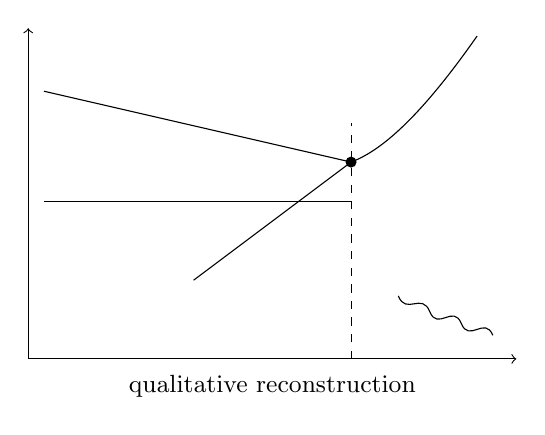
\begin{tikzpicture}[scale=1.0]
\draw[->] (0,0) -- (0,4.2);
\draw[->] (0,0) -- (6.2,0);
\draw[dashed] (4.1,0) -- (4.1,3.0);
\fill (4.1,2.5) circle (0.07);
\draw (0.2,3.4) -- (4.1,2.5);
\draw (0.2,2.0) -- (4.1,2.0);
\draw (2.1,1.0) -- (4.1,2.5);
\draw (4.1,2.5) .. controls (4.5,2.65) and (5.0,3.1) .. (5.7,4.1);
\draw (4.7,0.8) .. controls (4.8,0.55) and (5.0,0.85) .. (5.1,0.6)
      .. controls (5.2,0.35) and (5.4,0.7) .. (5.5,0.45)
      .. controls (5.6,0.2) and (5.8,0.55) .. (5.9,0.3);
\node at (3.1,-0.35) {\small qualitative reconstruction};
\end{tikzpicture}
\caption{A cautious TikZ reconstruction of the qualitative structure of the sketch: several branches, a marked threshold, a dashed guide, and the steep rise on the right. No exact labels are being asserted.}
\end{figure}

From here the lecture gives one of its most memorable estimates. A linear accelerator gains energy roughly linearly with its size. If \(100\,\mathrm{GeV}\) takes of order a few miles at SLAC, then \(10^{19}\,\mathrm{GeV}\) requires a machine larger by roughly \(10^{17}\). That is not a terrestrial machine. It is a galactic one. And even that is not enough, because an accelerator also needs luminosity. To probe Planckian distance scales one does not aim particles with Planck precision; one sends enormous numbers of particles at one another so that some collisions occur at the required impact parameters. The fuel bill, in the lecture's joking but pointed estimate, becomes astronomical. The conclusion is direct: a genuinely direct experimental probe of Planckian string physics is fantastically remote.

The same line of reasoning constrains extra dimensions. If extra dimensions were large enough to be explored at modest energies, ordinary quantum field theory would already have broken down. Since it seems to work extremely well out to very short distances, the extra dimensions, if present, must be tiny. And if one tries to make them much smaller than the Planck length, the corresponding mass scale becomes trans-Planckian and one slides back into the black-hole problem. So even the size of the extra dimensions is hemmed in by the same logic.

\section{The Easy Version of Why Twenty-Six Dimensions Appear}

After the break the lecture restarts very deliberately. Susskind says that the real mathematics of string theory lies in conformal transformations, but that he has only time to give what he calls the easy version of why bosonic string theory has twenty-six dimensions. He warns us in advance: the easy version is not easy, it is not satisfying, but it is historically important and it is correct.

The new starting point is the open string. We want the first excited state to be massless, because in the old bosonic string that is the candidate photon. Therefore the ground state must sit one unit lower in mass squared:
\begin{equation}
m_{\text{ground}}^{2}=-1.
\end{equation}
Then one unit of excitation raises it to zero mass squared. The existence of the tachyonic ground state is acknowledged and set aside; the lecture's question is narrower. Where does this \(-1\) come from?

The obvious place to look is the zero-point energy of the string oscillators.

\begin{figure}[t]
\centering

\includegraphics[width=0.70\textwidth]{lecture_05_figure_04.png}
\caption{Vacuum annihilation condition and ground-state equation. The board is partly obscured, but the stable content is clear: a vacuum condition, a coordinate-space differential equation, and the Gaussian ground-state form.}
\end{figure}

The board shows the familiar oscillator logic. In operator language the vacuum is defined by
\begin{equation}
a^-|0\rangle=0.
\end{equation}
In coordinate space this becomes, in cleaned form,
\begin{equation}
\left(x-\frac{\partial}{\partial x}\right)\psi_{0}(x)=0,
\end{equation}
whose normalizable solution is the Gaussian
\begin{equation}
\psi_{0}(x)\propto e^{-x^{2}/2}.
\end{equation}
So the ground state is not a state of zero energy; it already carries the usual zero-point contribution.

For the string, the \(n\)th oscillation mode has frequency
\begin{equation}
\omega_{n}=n.
\end{equation}
Therefore the ground-state energy of that single oscillator is
\begin{equation}
E_{0,n}=\frac{1}{2}\omega_{n}=\frac{n}{2}.
\end{equation}
Adding all the oscillators would seem to give
\begin{equation}
E_{0}^{\text{formal}}=\frac{1}{2}\sum_{n=1}^{\infty}n.
\end{equation}

Now the conceptual obstacle is in plain sight. Every term is positive. How could a sum of positive zero-point energies possibly produce the negative shift needed to place the photon one level above the ground state? This is the hinge of the second act of the lecture.

\section{Zero-Point Energy, Light-Cone Energy, and the Intercept Puzzle}

\subsection{Question \& Answer}

\paragraph{How can a sum of positive zero-point energies produce the negative ground-state shift needed for the photon?}

Susskind's answer is not to manipulate the sum immediately. First he says that we have to remember what quantity is actually being identified with \(m^{2}\). The relevant object is not the total energy of the boosted string, because the total energy contains an uninteresting piece: the large overall longitudinal momentum.

This is why he backs up and rewrites the energy of a very fast system.

\begin{figure}[t]
\centering

\includegraphics[width=0.72\textwidth]{lecture_05_figure_05.png}
\caption{Subtracting longitudinal momentum from the energy. The board writes the large-\(P\) expansion first and then, on the next line, forms \(E-P\) to isolate the internal piece.}
\end{figure}

In the infinite-momentum limit one has
\begin{equation}
E=P+\frac{m^{2}}{2P}.
\end{equation}
The first term is just the overall motion down the \(z\)-axis. It is conserved, and for internal spectroscopy we do not care about it. So we subtract it:
\begin{equation}
E-P=\frac{m^{2}}{2P}.
\end{equation}
Then we multiply by \(2P\) and recover the invariant quantity,
\begin{equation}
2P(E-P)=m^{2}.
\end{equation}
The board photograph shows only the left-hand side of the subtraction step; the right-hand side is the natural completion of the lecture's algebra.

Susskind justifies this physically by time dilation. A fast-moving composite system carries a large overall energy, but its internal motions run slowly. The lecture illustrates the point with an atom: as the atom is boosted, the total energy grows, but the internal level splittings shrink. Those splittings scale like \(1/P\). Multiplying by \(2P\) removes that trivial kinematic suppression and leaves the mass squared.

So the zero-point problem changes form. We do not literally need the raw sum of oscillator energies to equal \(-1\). What we need is that, once the trivial longitudinal piece has been separated away, the internal energy should behave like
\begin{equation}
-1+\text{an infinite additive constant}.
\end{equation}
That infinite constant is not pleasant, and Susskind says so explicitly. But it is also not new. The boosted energy already contains huge additive pieces associated with the overall motion, and the divergence we are about to uncover can be absorbed into such an already-present constant. The interesting part is the finite remainder.

\section{Regulating \(1+2+3+\cdots\), Then Counting Dimensions}

Now comes the mathematical trick. The board algebra in the lecture is lively and partly corrected on the fly, so the best way to preserve the argument is to keep the strategy and write the cleaned formulas.

Introduce a regulator \(\epsilon>0\) and replace the formal sum by
\begin{equation}
S(\epsilon)=\sum_{n=1}^{\infty} n e^{-n\epsilon}.
\end{equation}
For \(\epsilon>0\) this converges, and when \(\epsilon\to 0^{+}\) it tends back toward the original divergent series. The point is to separate from it an infinite part and a finite part.

The first step is the derivative trick. The photographed frame does not show the crucial minus sign clearly, but the transcript makes clear that it must be there:
\begin{equation}
S(\epsilon)
=
-\frac{\partial}{\partial\epsilon}\sum_{n=1}^{\infty} e^{-n\epsilon}.
\end{equation}
The inner sum is geometric:
\begin{equation}
\sum_{n=1}^{\infty} e^{-n\epsilon}
=
e^{-\epsilon}+e^{-2\epsilon}+e^{-3\epsilon}+\cdots
=
\frac{e^{-\epsilon}}{1-e^{-\epsilon}}.
\end{equation}
Therefore
\begin{equation}
S(\epsilon)
=
-\frac{\partial}{\partial\epsilon}
\left(
\frac{e^{-\epsilon}}{1-e^{-\epsilon}}
\right).
\end{equation}

Since we only care about the limit of small \(\epsilon\), we expand:
\begin{equation}
\frac{e^{-\epsilon}}{1-e^{-\epsilon}}
=
\frac{1}{\epsilon}-\frac{1}{2}+\frac{\epsilon}{12}+O(\epsilon^{3}).
\end{equation}
Differentiating then gives
\begin{equation}
\sum_{n=1}^{\infty} n e^{-n\epsilon}
=
\frac{1}{\epsilon^{2}}-\frac{1}{12}+O(\epsilon^{2}).
\end{equation}

This is the central result of the calculation. The regulated version of \(1+2+3+\cdots\) breaks into
\begin{equation}
\underbrace{\frac{1}{\epsilon^{2}}}_{\text{divergent constant}}
\;+\;
\underbrace{\left(-\frac{1}{12}\right)}_{\text{finite part}}
\;+\;
O(\epsilon^{2}).
\end{equation}
The lecture's point is not that \(1+2+3+\cdots\) converges in the ordinary sense to \(-1/12\). The point is that after the correct regularization, and after one agrees to absorb the divergent constant into an already-existing infinite piece of the boosted energy, the finite remainder is
\begin{equation}
-\frac{1}{12}.
\end{equation}

But the string zero-point energy has an extra factor of \(1/2\), coming from \(\frac{1}{2}\omega_{n}\). So one transverse oscillator contributes
\begin{equation}
E_{0}^{\text{per transverse oscillator}}=-\frac{1}{24}.
\end{equation}

Now the dimension counting is immediate. If there were only two transverse oscillation directions, as in the naive picture with \(x\)- and \(y\)-oscillators, then the ground-state shift would be only
\begin{equation}
2\left(-\frac{1}{24}\right)=-\frac{1}{12},
\end{equation}
which is nowhere near the \(-1\) required for the open string. So the lecture makes the historical leap: suppose there are \(D_{\perp}\) transverse directions. Then
\begin{equation}
E_{0}^{\text{open}}=-\frac{D_{\perp}}{24}.
\end{equation}
To get the massless photon one unit above the ground state, we require
\begin{equation}
-\frac{D_{\perp}}{24}=-1,
\end{equation}
and therefore
\begin{equation}
D_{\perp}=24.
\end{equation}
Adding the longitudinal spatial direction and time gives the total spacetime dimension
\begin{equation}
D=D_{\perp}+2=26.
\end{equation}

The lecture then goes back to the closed string. There one needs two excitations to reach the massless spin-two state. So the ground state should sit at \(-2\), not \(-1\). At first that sounds like trouble, because \(24\) transverse directions only give \(-1\). But the closed string has both left-moving and right-moving oscillators, so the zero-point contribution doubles:
\begin{equation}
E_{0}^{\text{closed}}
=
2\left(-\frac{D_{\perp}}{24}\right).
\end{equation}
With \(D_{\perp}=24\) this becomes
\begin{equation}
E_{0}^{\text{closed}}=-2,
\end{equation}
which is exactly what is needed.

This is the easy version of \(D=26\). It is historically close to the way the result first appeared. People noticed that one level above the ground state sat a spin-one particle with only the two polarizations appropriate to a massless vector, and that forced attention onto the zero-point shift. From there the number \(24\) of transverse oscillators, hence \(26\) spacetime dimensions, emerged rather quickly. But Susskind does not let the audience walk away thinking the matter is conceptually settled. This argument is real, but it is not the deep reason. The deeper reason, deferred to the next lecture, is conformal invariance.

\section{Summary}

The lecture begins by correcting a simple omission, units, and ends with the old bosonic dimension count \(D=26\). The bridge between those two endpoints is the tension. A stretched string behaves like a spring, so there is one natural scale \(T=\sqrt{k}\), and in the infinite-momentum description that scale governs increments of mass squared. For fundamental strings that scale lies near the Planck regime, which is why the strings are tiny, the excitation energies huge, and direct tests so remote. After the break the lecture turns that same viewpoint onto the bosonic ground state: the positive zero-point energies are reorganized in light-cone variables, regulated by an \(\epsilon\)-trick, and split into an infinite constant plus a finite remainder. The remainder gives \(-1/24\) per transverse oscillator, and from that one reaches \(24\) transverse directions for the open string and \(26\) spacetime dimensions in all, with the closed-string case fitting by left-right doubling. The chapter closes where the lecture closes: this is the easy version, historically illuminating but not conceptually final. The real explanation begins with conformal invariance.